To perform this evaluation, a 10-fold cross-validation is performed in
order to assess the decision tree's accuracy. Using the cross-validation an
average error of the ten estimates is 10\% was discovered. 

Having the 10-fold cross validation calculated on the training set, the
classified results are used to generate a confusion matrix.

To be more specific, the 10 predicted subsets are concatenated and passed along
with the actual target labels into a function responsible for the calculation of
the confusion matrix. The calculated confusion matrix can be seen in
figure~\ref{fig:confusionMatrix}.

\include*{confusion_matrix}

From this matrix it can be observed that the correct classifications for each
class are on the matrix's diagonal. This matrix clearly shows that the
'Surprise' class is identified correctly. On the other hand, for the rest classes there are some misclassified examples. 

For the calculation of the precision and the recall rates per class, two
formulas have been used. Those formulas use information from the confusion
matrix to calculate those two rates.

The recall and precision rates are being presented in the table~\ref{fig:averageRecall}
\include*{average_recall_precision}

The figure~\ref{fig:confisionMatixCalc} is an example of a small confusion matrix.
It can been used to show the rates may be calculated.

\begin{figure}[h]
    \centering
    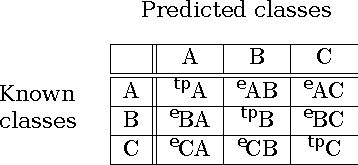
\includegraphics[width=0.3\textwidth]{confusionMatrixCalc.pdf}
    \caption{A simple confusion matrix}
    \label{fig:confisionMatixCalc}
\end{figure}

The recall and the precision can be derived from the confusion matrix by
applying the following formulas:

Precision\textsubscript{A} = tp\textsubscript{A}/(tp\textsubscript{A}+e\textsubscript{BA}+e\textsubscript{CA})

Recall\textsubscript{A} = tp\textsubscript{A}/(tp\textsubscript{A}+e\textsubscript{AB}+e\textsubscript{AC})

The precision and recall rates, along with the F\textsubscript{1} measure, reflect our previous conclusions for the classes.
